\chapter{Results}
\chlab{results}

In the user studies, a lot of different types of data has been created. First, graphical representations of most observations from the user action log can be found in \appref{graphs}. In that same chapter, the outcomes of the \verb|SUS| and \verb|UMUX| questions that were asked in the questionnaire can also be found. \Appref{comments} contains all answers to the open questions, including general comments about the system, the preferred version and suggestions for improvement.

This chapter will contain the important and most interesting results obtained in the user studies. Each result will shortly be discussed, and further analysed in \chref{discussion}.


\section{Action log results}
From the logging system that was built into \oframp{} for the user studies, a wide range of information can be gathered, spanning from the load time and the number of clicks on atom 5 to the selected conflict solutions and resulting parameterisation. This section contains the most interesting results that can be retrieved from the action log.

\subsection{Time required}
First of all, it is interesting to see in what version users spent the most time to fully parameterise the molecules. \Figref{graph_time_1} shows the total time that was required for both the first and second set of molecules, in both the naive and smart version of \oframp. What can be seen here is that, for both the first and second set of molecules, users needed more time to complete the parameterisation using the naive version. Users who started with the naive version used the most time overall, with a median total time of around 300 seconds, after which those same users spent the least time on the smart version, where the median time value is around 100 seconds. At around 200 and 150 seconds, one can find the median times required by the users who did the naive version second and the smart version first respectively.

\begin{figure}[h!]
\center
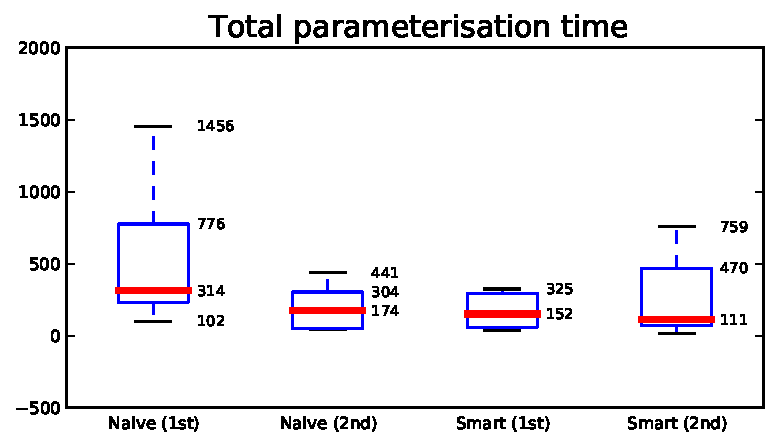
\includegraphics[width=.6\textwidth]{img/graphs/1a_02.pdf}
\caption{Total parameterisation time for the two versions in the two orders.}
\figlab{graph_time_1}
\end{figure}

The total time used to parameterise the first and second sets of molecules can be used to determine what version of \oframp{} is the most time-consuming. However, as both sets of molecules have slightly varying molecule sizes, it may be more interesting to look at the average time that was required per atom. This can be seen in \figref{graph_time_2}.

\begin{figure}[h!]
\center
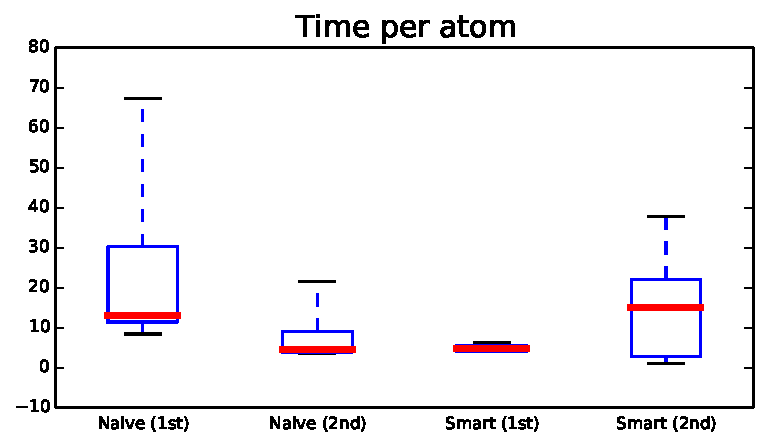
\includegraphics[width=.6\textwidth]{img/graphs/1a_03.pdf}
\caption{Average time per atom for the two versions in the two orders.}
\figlab{graph_time_2}
\end{figure}

What is interesting to see here, is the fact that, where in the total parameterisation time, the group that did the smart version second was done the fastest, its members have spent the most time on average per atom. When taking a closer look at \figref{graph_time_3} and \figref{graph_time_4}, which show the average time per atom required for all molecules separately, this difference appears to be caused completely by the excessive amount of time users spent on parameterising molecule 13913 in the smart version, which is the first molecule users got to parameterise after they have completed the naive version. Even more interesting to see is the fact that most users spent more time parameterising this 11-atom molecule than on the larger 77-atom molecule 17738.

\begin{figure}[h!]
\centering
\begin{subfigure}[t]{0.48\textwidth}
\centering
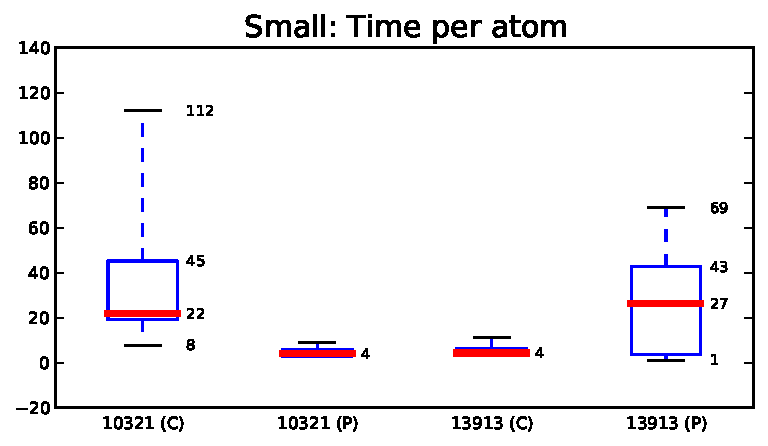
\includegraphics[width=\textwidth]{img/graphs/1c_03.pdf}
\caption{Smaller molecules.}
\figlab{graph_time_3}
\end{subfigure}%
~
\begin{subfigure}[t]{0.48\textwidth}
\centering
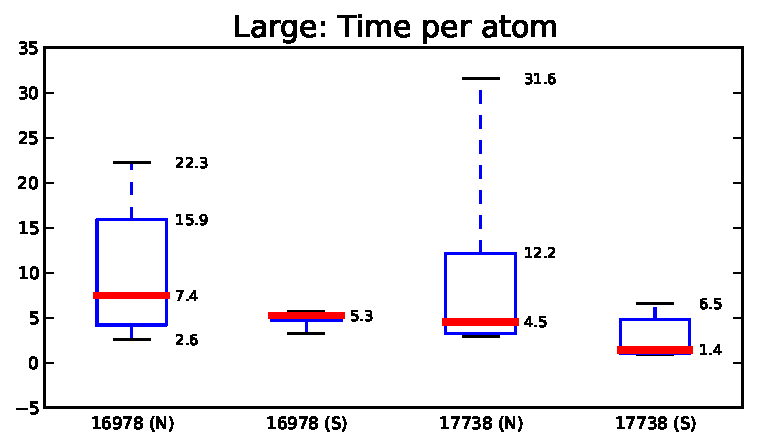
\includegraphics[width=\textwidth]{img/graphs/1d_03.pdf}
\caption{Larger molecules.}
\figlab{graph_time_4}
\end{subfigure}
\caption{Average time per atom for all molecules in the two orders.}
\figlab{graph_time_34}
\end{figure}

It is hard to say what exactly is causing this difference. It is possible that, after using the naive version, it is hard to get used to the smart version, which is way more restrictive as to what a user can do. However, this difference is not present when switching from the smart to the naive version. This can either mean that this switch is easier to make, or that there must be a different cause of the large time difference.

Another possible explanation for the large increase in time required for parameterising molecule 13913 is that there may not be really good matching fragments, enforcing the user to browse through many of them before being able to select the best one. This is better facilitated by the naive version of the tool, and can potentially have the extreme effects that are observed here.

Apart from molecule 13913, \figref{graph_time_34} shows that finishing a parameterisation using the naive version of \oframp{} requires more time than using the smart one. It is also clear that the time required is much more constant, and, with an overall average of around 7 seconds per atom, overall still the fastest, compared to 10 seconds for the naive version.


\subsection{Parameterisation rating}
Not only the time required by the parameterisation tool is important to determine which interaction design is the best, the quality of the result is also of great importance. As discussed in \secref{analysis}, there are two ways of calculating this quality rating. First, the total difference between the charge found by the user and the charge present in the ATB can be found, as shown in \figref{graph_rating_1}. As this difference can easily be observed and corrected by the user, it would be expected that it would be relatively close to 0. This, however, turns out not to be the case. Especially in the smart version of \oframp, the charge difference can get quite high, and is greater than the charge difference for the naive version in any case.

\begin{figure}[h!]
\center
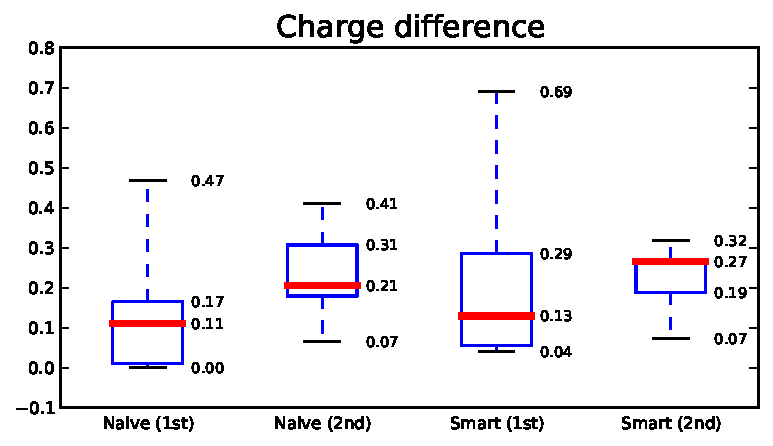
\includegraphics[width=.6\textwidth]{img/graphs/1a_00.pdf}
\caption{Total charge difference for the two versions in the two orders.}
\figlab{graph_rating_1}
\end{figure}

What is also interesting to note here is the fact that, for both the naive and the smart versions of \oframp, the total charge difference is higher for the second set of molecules. This may indicate that these molecules are harder to parameterise, or that there are no good matching fragments for those molecules available. However, it may also indicate that users were starting to lose their concentration, or were confused due to the switch from one version to another.

Where the difference in the total molecule charge can mainly be used to assess user performance, the correctness of the parameterisation can better be measured using the per-atom charge differences. \Figref{graph_rating_2} shows these differences for the first and second set of molecules, both for the naive and smart version of \oframp. As can be seen in that graph, charge differences are, again, smaller for the naive version than they are for the smart version.

\begin{figure}[h!]
\center
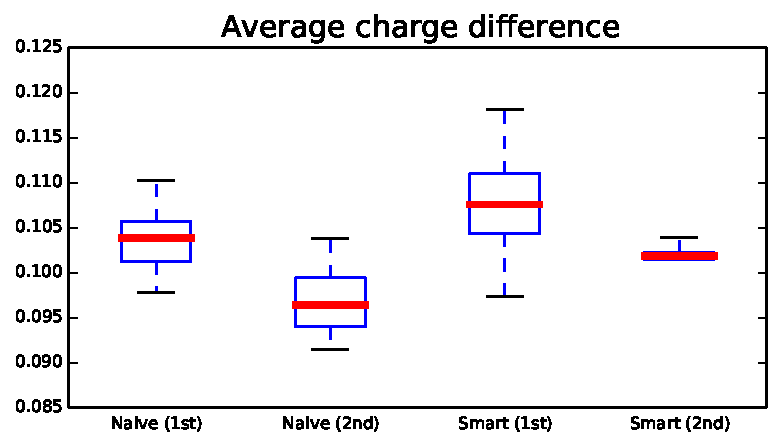
\includegraphics[width=.6\textwidth]{img/graphs/1a_01.pdf}
\caption{Average charge difference per atom for the two versions in the two orders.}
\figlab{graph_rating_2}
\end{figure}

In contrast to the total charge differences though, the average charge differences for the second set of molecules are smaller than those for the first set. This suggests the opposite of what was concluded from \figref{graph_rating_1}: the second set of molecules may be easier to parameterise, or there may be better matching fragments available. This suggestion is more probable, as for the total charge difference a negative offset between two atom charges can be compensated by a positive offset in two others, which is not the case for the per-atom difference.

As can be seen in \figref{graph_rating_34}, the naive version of \oframp{} scores better for all individual molecules. What can also be seen there is the fact that, even on average, the charge differences are bigger for the larger molecules than for the smaller ones. Unfortunately, there is no obvious explanation for this. Probably, larger fragments are used for the larger molecules. When one of those fragments is wrong, it quickly adds up to the atom charge difference. On the other hand, it is also possible that users felt more comfortable selecting small fragments, which are generally worse matches than the large ones, due to less atoms matching between the two molecules.

\begin{figure}[h!]
\centering
\begin{subfigure}[t]{0.48\textwidth}
\centering
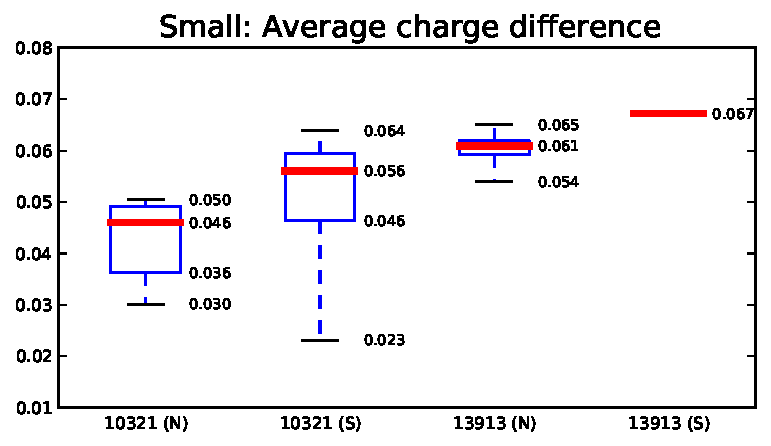
\includegraphics[width=\textwidth]{img/graphs/1c_01.pdf}
\caption{Smaller molecules.}
\figlab{graph_rating_3}
\end{subfigure}%
~
\begin{subfigure}[t]{0.48\textwidth}
\centering
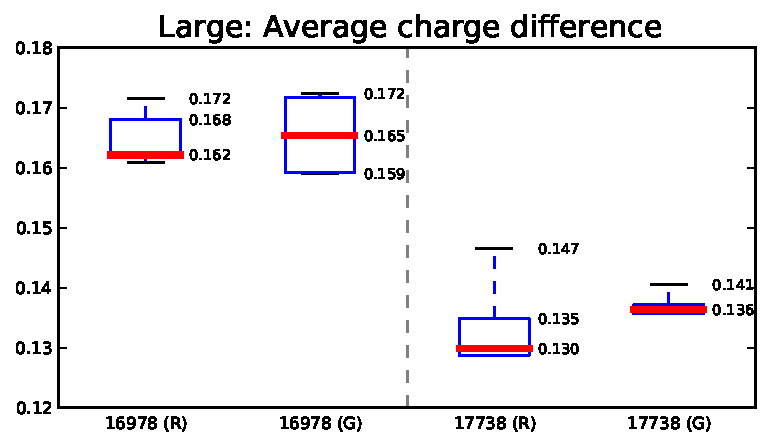
\includegraphics[width=\textwidth]{img/graphs/1d_01.pdf}
\caption{Larger molecules.}
\figlab{graph_rating_4}
\end{subfigure}
\caption{Average charge difference per atom for all molecules in the two orders.}
\figlab{graph_rating_34}
\end{figure}

\subsection{Other results}
Besides the time required to complete the parameterisation and its rating, some other interesting things were observed in the user studies. First of all, there appears to be a great correlation between the version of \oframp{} that is used and the amount of actions a user needs to undo, as can be seen in \figref{graph_undo}. Where in the naive version, users practically do not undo any action, there are extreme cases where a user needed to undo over a hundred times in the smart version. This difference can be explained by the fact that users of the smart version have to undo accidentally rejected fragments, or may use a combination of reject and undo actions to compare various fragments.

\begin{figure}[h!]
\center
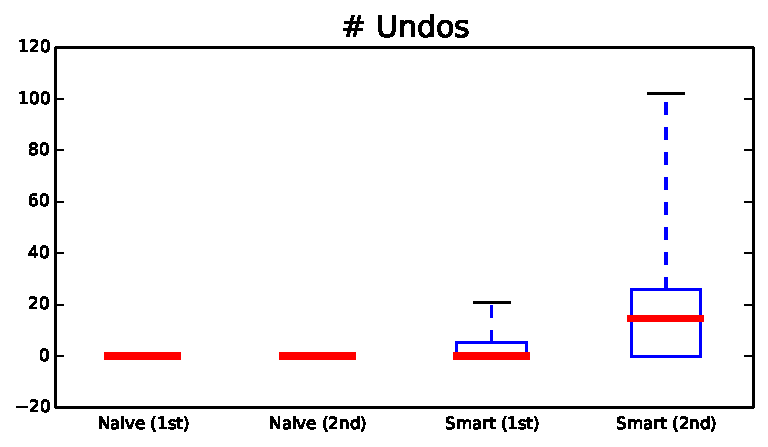
\includegraphics[width=.6\textwidth]{img/graphs/1a_10.pdf}
\caption{Number of undo actions for the two versions in the two orders.}
\figlab{graph_undo}
\end{figure}

As can be seen in \figref{graph_clicks}, a few more clicks are required to complete a parameterisation in the smart version of the tool, then there are in the naive version. Nevertheless, the medians are not too far apart, so it is not really possible to draw any conclusions from this. It is interesting to see, however, that even though the smart version of \oframp{} requires less user interaction, is does not require less, and possibly even more clicks to complete a parameterisation.

\begin{figure}[h!]
\center
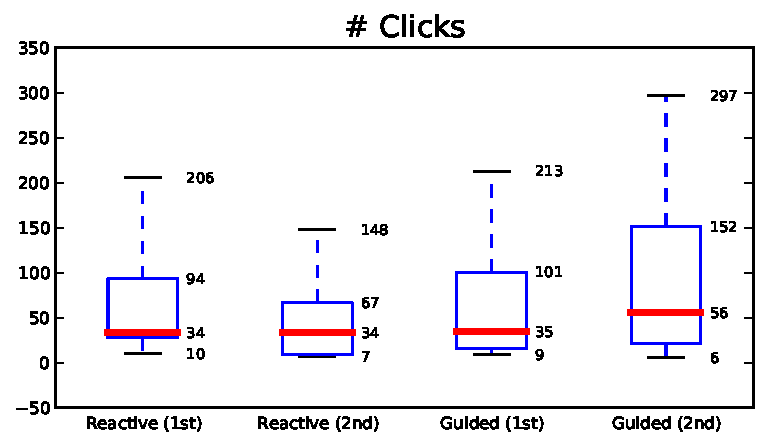
\includegraphics[width=.6\textwidth]{img/graphs/1a_04.pdf}
\caption{Total number of clicks for the two versions in the two orders.}
\figlab{graph_clicks}
\end{figure}

\Figref{graph_help} shows that not many users had to consult the help pages during the parameterisation process. Furthermore, no users checked the help pages in their second version of the system. This can mean that either they did not know there were different versions of the help pages as well, or they did not need it any more. The fact that most users did not go to the help pages at all suggests that the tool is intuitive to use, and that taking the demo provides enough information to be able to use \oframp.

\begin{figure}[h!]
\center
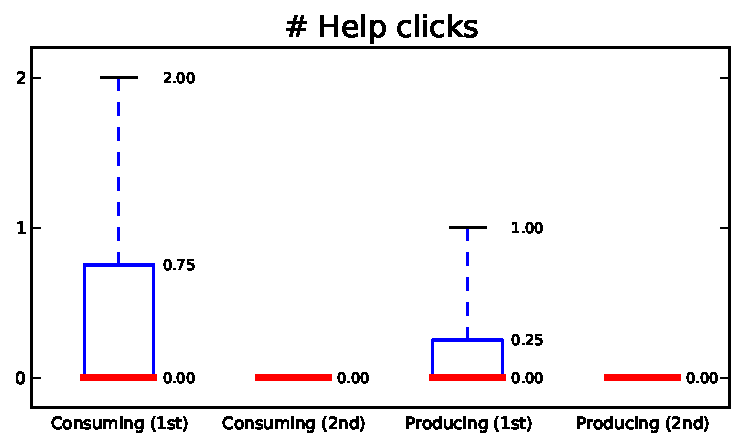
\includegraphics[width=.6\textwidth]{img/graphs/1b_01.pdf}
\caption{Total number of clicks on the help button for the two versions in the two orders.}
\figlab{graph_help}
\end{figure}

There are also a few things users did not do at all. They were not required or instructed to use every aspect of \oframp, but it was expected that they would at least try some of the more advanced features. First, none of the users used any of the available keyboard shortcuts. Although all actions for which a keyboard shortcut exists can also be completed using a single mouse click, it was expected that some users would find it beneficial to use keyboard shortcuts for some actions, but this turned out not to be the case.

Furthermore, and more surprisingly, none of the users manually edited a single atom charge. Again, they were not specifically instructed to do so, but they were made aware of the possibility of doing this, and instructed to make the parameterisation as good as possible. Possibly, users were unable to locate the position of the charge edit fields, but no comments about that have been made. Probably, they just did not feel the need of it, or thought their parameterisation was perfect the way it was.

\subsection{Correlations}
From the data gathered from the log files, it is interesting to see if there is any correlation between the rating of the outcome and any other parameter. \Figref{graph_correlation} shows four presumed possible correlations, with data points for both the naive and the smart version of \oframp. Trend lines have been plotted - a cyan one for the naive version and a magenta line for the smart - to help identifying if there is any correlation.

\begin{figure}[h!]
\centering
\begin{subfigure}[t]{0.48\textwidth}
\centering
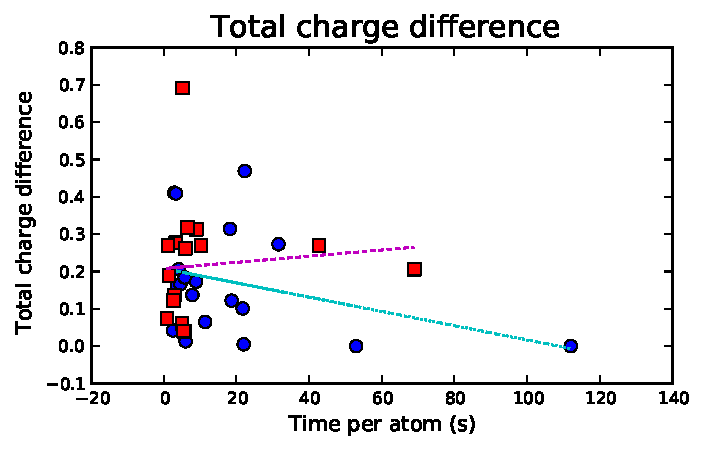
\includegraphics[width=\textwidth]{img/graphs/3a_01.pdf}
\caption{Total charge difference in relation to the average time used per atom.}
\figlab{graph_correlation_1}
\end{subfigure}%
~
\begin{subfigure}[t]{0.48\textwidth}
\centering
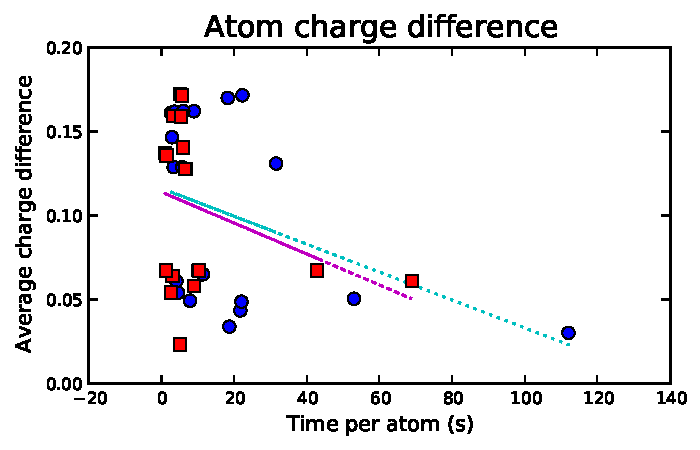
\includegraphics[width=\textwidth]{img/graphs/3a_00.pdf}
\caption{Average charge difference per atom in relation to the average time used per atom.}
\figlab{graph_correlation_2}
\end{subfigure}%
\\[1em]
\begin{subfigure}[t]{0.48\textwidth}
\centering
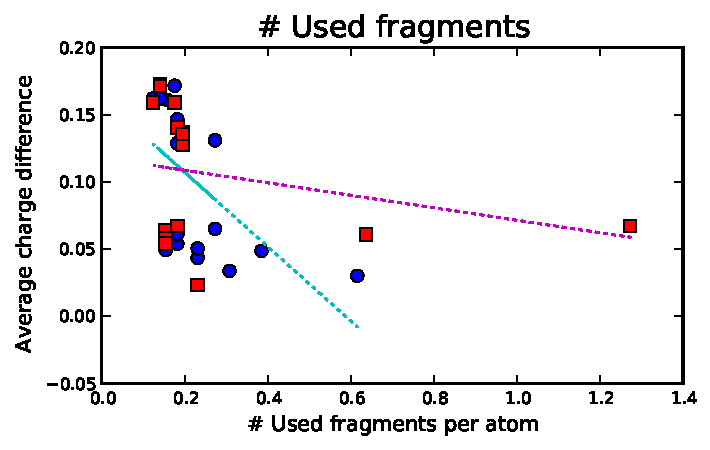
\includegraphics[width=\textwidth]{img/graphs/3a_02.pdf}
\caption{Average charge difference per atom in relation to the number of used fragments per atom.}
\figlab{graph_correlation_3}
\end{subfigure}%
~
\begin{subfigure}[t]{0.48\textwidth}
\centering
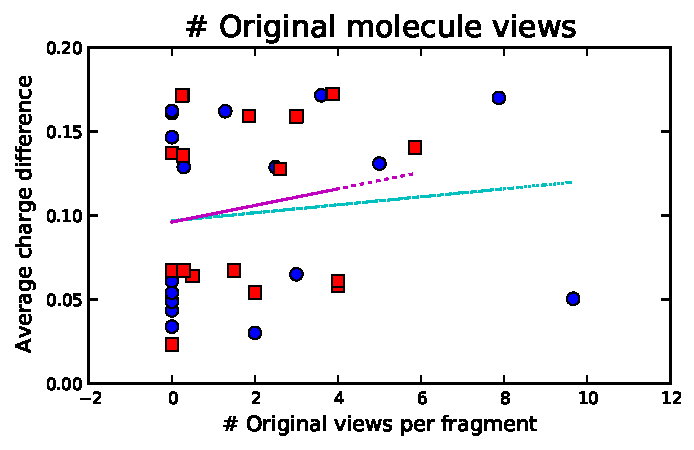
\includegraphics[width=\textwidth]{img/graphs/3a_03.pdf}
\caption{Average charge difference per atom in relation to the number of original molecule views per selected fragment.}
\figlab{graph_correlation_4}
\end{subfigure}
\caption{Presumed correlations between user studies outcomes. The blue circles are data points gathered from the naive version, the red squares come from the smart version.}
\figlab{graph_correlation}
\end{figure}

However, as one can see almost immediately, there does not appear to be any correlation between any of the graphs shown in \figref{graph_correlation}. Even when the most extreme outliers are removed, the data points are still widely scattered and no correlation can be observed.

When taking a look at \figref{graph_correlation_1} and \figref{graph_correlation_2}, it does appear that the parameterisations the most time has been spent on are amongst the best rated. However, they are not \emph{the} best rated, and may just be outliers as they are found in isolation from the rest of the points. Furthermore, for the smart version, the users that spent the most time are not performing better than average, but these may still be outliers. A larger test group would be needed to confirm the (lack of) correlation here.

Just like is the case for the charge differences, the extremes in the number of used fragments are among the best results~(see \figref{graph_correlation_3}). However, it may also be the case here that these points are just outliers, and more experimentation is needed to be able to observe any real trend.

For the number of original molecule views, the results are the most widespread~(see \figref{graph_correlation_4}). It appears that viewing many original molecules has absolutely no effect on the quality of the parameterisation result. Furthermore, the best results for both the naive and smart version of \oframp{} are obtained by users who did not check a single original molecule. This is an interesting observation, as it is believed that, in order to judge if a fragment is a good match, one needs to see the fragment in the context of its originating molecule.


\section{Questionnaire outcomes}
\nlipsum

\subsection{\texttt{SUS} / \texttt{UMUX} results}
\nlipsum

\begin{figure}[h!]
\center
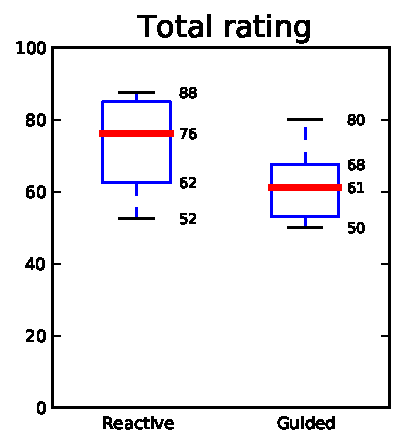
\includegraphics[width=.3\textwidth]{img/graphs/4a_10.pdf}
\caption{Average rating for the two versions.}
\figlab{graph_rating_1}
\end{figure}

\begin{figure}[h!]
\center
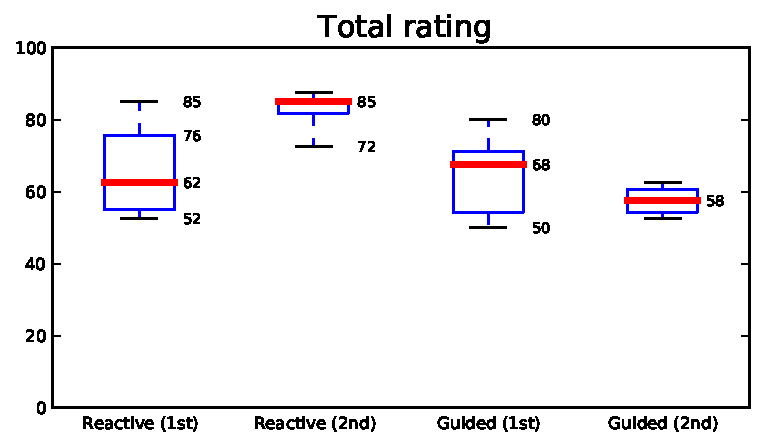
\includegraphics[width=.6\textwidth]{img/graphs/4b_10.pdf}
\caption{Average rating for the two versions in the two orders.}
\figlab{graph_rating_2}
\end{figure}

\begin{figure}[h!]
\centering
\begin{subfigure}[t]{0.32\textwidth}
\centering
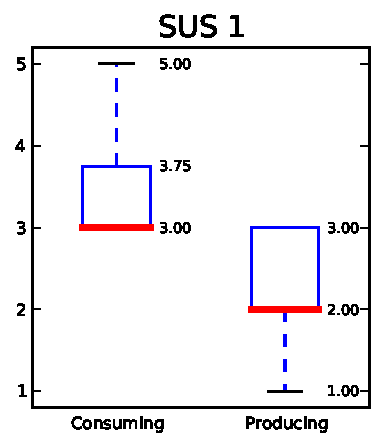
\includegraphics[width=\textwidth]{img/graphs/4a_00.pdf}
\caption{Rating of \texttt{SUS1}.}
\figlab{graph_rating_3}
\end{subfigure}%
~
\begin{subfigure}[t]{0.32\textwidth}
\centering
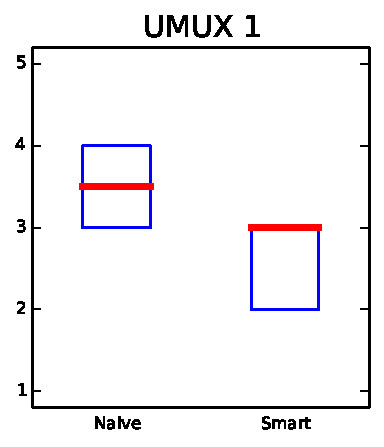
\includegraphics[width=\textwidth]{img/graphs/4a_01.pdf}
\caption{Rating of \texttt{UMUX1}.}
\figlab{graph_rating_4}
\end{subfigure}%
~
\begin{subfigure}[t]{0.32\textwidth}
\centering
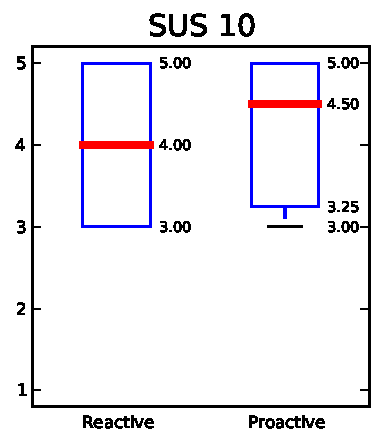
\includegraphics[width=\textwidth]{img/graphs/4a_09.pdf}
\caption{Rating of \texttt{SUS10}.}
\figlab{graph_rating_5}
\end{subfigure}
\caption{Selected ratings for the two versions of \oframp.}
\figlab{graph_rating_345}
\end{figure}


\subsection{Comments}
\nlipsum
